\documentclass[acmsmall,screen,review,anonymous]{acmart}
\usepackage[utf8]{inputenc} % Required for inputting international characters
\usepackage[T1]{fontenc} % Output font encoding for international characters

\usepackage{palatino} % Use the Palatino font by default
% Using BibTeX with acmart's built-in natbib support


% \usepackage[a4paper,margin=1in]{geometry}
\usepackage{float}
\usepackage[ruled,linesnumbered]{algorithm2e}
\SetKwInput{KwIn}{Input}
\SetKwInput{KwOut}{Output}
% \usepackage[hidelinks]{hyperref}
\usepackage{amsmath}
\let\Bbbk\relax  % Prevent conflict with newtx fonts
\usepackage{amssymb}
\usepackage{balance}
\usepackage{booktabs}
\usepackage{cancel}
\usepackage{caption}
\usepackage{colortbl}  % for coloring table rules
\usepackage{enumitem}
\usepackage{fancybox}
\usepackage{framed}
\usepackage{graphicx}
\usepackage[htt]{hyphenat} % globally allow hyphenations to break lines
\usepackage{listings}
\usepackage{makecell}
\usepackage{multirow}
\usepackage{pifont}    % provides the \ding command
\usepackage{pdflscape} % for landscape env
\usepackage{subcaption} % supercedes subfig package
\usepackage{textcomp}
\usepackage{tikz}
\usetikzlibrary{positioning, shapes.geometric, fit, calc}
\usepackage{xurl}
\usepackage{xcolor}
\usepackage{xspace}

% Reduce hyphenation in normal text (higher = less hyphenation)
\hyphenpenalty=2000
\exhyphenpenalty=2000

% Make LaTeX more willing to place floats on text pages
\renewcommand{\topfraction}{0.9}
\renewcommand{\bottomfraction}{0.9}
\renewcommand{\textfraction}{0.1}
\renewcommand{\floatpagefraction}{0.7}

\newcommand{\spoilsport}{\textsc{Spoilsport}\xspace}
\newcommand{\approach}{\textsc{GoalSeeker}\xspace}

% Thesis sub-questions (update text as needed)
\newcommand{\sqIII}{How can goal-directed analysis uncover rug pull mechanics?\xspace}

% Roles
\newcommand{\holder}{\textit{Token Holder}\xspace}
\newcommand{\owner}{\textit{Contract Owner}\xspace}

% Goals
\newcommand{\maxsupply}{\textit{maxSupply}\xspace}
\newcommand{\minsupply}{\textit{minSupply}\xspace}
\newcommand{\maxowned}{\textit{maxOwned}\xspace}
\newcommand{\liquidity}{\textit{liquidity}\xspace}

% Feature formatting (for contract features like mint, burn, etc.)
\newcommand{\feature}[1]{\texttt{#1}}

% Revision marker (can be used to highlight revisions; currently just passes through)
\newcommand{\rev}[1]{#1}

% Constants
\newcommand{\numcontracts}{132\xspace}

\newenvironment{results}{\begin{framed}\small\centering\it}{\end{framed}}
\newenvironment{result}{\begin{framed}\small\centering\it}{\end{framed}}



\title{Goal-Directed Fuzzing for ERC-20 Rug Pulls}

\begin{abstract}
    Rug pulls are a prominent source of DeFi fraud, allowing malicious actors to profit at the expense of investors.
We investigate whether specifications of generic ERC-20 user roles (e.g., \holder) and goals (e.g., \maxowned) can be used to surface rug pull mechanisms in a high-level dataset of 1,376 known rug pull contracts.
These roles and goals are defined in terms of the contracts' state variables and transaction history, without tailoring to particularities of rug pulls.
To this end, we implement the \spoilsport fuzzer to automatically discover 2,731 transaction sequences which violated user goals.
Through manual analysis, we find that 83.6\% of rug pull types had corresponding violated goals.
The goal violations also revealed 105 misclassifications in the original dataset and unearthed 964 additional rug pull mechanisms that were not labelled in the dataset.
These goal-violating transaction sequences further serve as examples of how rug pulls may be performed for the given contracts.
Additionally, we develop a novel methodology for finding usage-realistic states upon which to begin our goal violation search, successfully initializing 1,324 (96.3\%) of our target contracts prior to beginning the search.
\end{abstract}

\begin{document}
\maketitle

Having developed and evaluated the \approach{} framework in \autoref{ch:goalseeker} in order to uncover risks to end-user goals, we now apply it to rug pulls, a prominent category of fraud in blockchain smart contracts.
This chapter addresses \textbf{SQ3} \sqIII{}
Here, we develop a goal-directed fuzzer which implements the \approach{} framework in order to run our evaluation.

Rug pulls are a prevalent category of fraud in which malicious actors launch a decentralized finance (DeFi) project and then abscond with investments, leaving investors with no financial value.
A recent study~\cite{defi-crime-map_jcs25} shows that at least USD644M was stolen through rug pulls through 2017-2022.
This fraud is often achieved through use of trap doors within smart contracts~\cite{SoKRugPull2025}, which are hidden or unintentional functionalities that enable the perpetrator to profit at the expense of investors.
For instance, a malicious developer may misleadingly name a \feature{mint} (token generation) feature as \feature{burn()} to imply token destruction functionality.

In this work, we investigate whether goal violations from a general ERC-20 specification can recover and enrich known rug pulls without tailoring the specification to rug pulls.
This is motivated by our observation that trap doors rely on end-user misunderstanding of smart contract implementation details to profit at the expense of these end-users.
Goal violations highlight scenarios in which end-user desires are thwarted.
This suggests that, through no additional specification effort for the goal violation discovery, the found violations may surface underlying mechanics of rug pulls.
We thus implement \spoilsport{}, a goal-directed fuzzer based on the \approach{} framework to investigate 1,376 known ERC-20 rug-pull contracts collected by prior work~\cite{SoKRugPull2025}.

Additionally, we develop an automated methodology for discovering meaningful starting states upon which to begin analysis.
A key challenge for goal analysis is to begin inspection at a usage-realistic starting state which resembles characteristics of the smart contract's intended usage.
For instance, when analyzing an ERC-20 contract, we would like to start from a state where the tokens are distributed to multiple users and at least one of them is liquid.
Existing fuzzers typically either rely on manual deployment scripts, fork full, potentially complex on-chain state or else search for states that are well-positioned for discovering security vulnerabilities, rather than usage-realism.
We address this by leveraging our fuzzer and role/goal semantics in order to specify state characteristics of such usage-realism and solving for a reachable state prior to beginning our goal analysis.

Our contributions are as follows:
\begin{enumerate}
    \item \textbf{Role/goal-based state initialization methodology:}
        We propose a declarative state initialization methodology based on \approach{} role/goal semantics.
        This allows for concise, natural specification of characteristics of a meaningful starting state.
    \item \textbf{\spoilsport Implementation:}
        We implement the \spoilsport{} goal-directed fuzzer and state initializer, which takes user-given specification in role/goal semantics to discover goal violations on a target contract.
        To evaluate this, we also compare results from the \spoilsport{} fuzzer with the \approach{} solver.
        \spoilsport{} discovers more (+38.3\%) goal violations in less time (~23x faster) on the same top ERC-20 contracts used in the initial \autoref{ch:goalseeker} evaluation.
    \item \textbf{Rug Pull Analysis:}
        We evaluate how well the surfaced ERC-20 goal violations retrieve mechanisms which aid in rug pulls within a corpus of 1,376 known rug pull contracts.
        For these, we successfully initialize 96.3\% of them to meaningful starting states in a mean of 1.54s.
        We then discovered 2,731 goal violations, with 83.6\% of contracts having goal violations which correspond to their labelled rug pull type and providing additional detail beyond the original labels.
\end{enumerate}
\section{Background}
\label{ss:sec:background}

\subsection{Ethereum Smart Contracts and Rug Pulls}
\smallskip
\noindent
\textbf{Ethereum Smart Contracts:}
    The Ethereum blockchain~\cite{EthereumWhitepaper} was launched in 2015, bringing with it Turing-complete smart contracts.
    Ethereum is currently the second largest public blockchain with a market capitalization exceeding USD349 billion~\cite{EthMarketCap} for its native Ether token.
    These smart contracts are generally written in the Solidity~\cite{Solidity} language and then compiled to bytecode targeting the Ethereum Virtual Machine, which has numerous popular implementations.

\smallskip
\noindent
\textbf{ERC-20 Tokens and Rug Pulls:}
ERC-20 tokens~\cite{ERC20TokenStandard} are the most popular standard in the Ethereum ecosystem.
These are fungible tokens, standardized for interoperability.
This standardization additionally allows them to be easily listed on decentralized exchanges (DEXs) such as Uniswap~\cite{uniswap_protocol}, which facilitate the exchange of tokens without the need for centralized authority.
They are also a popular target for rug pulls.

As highlighted by prior work~\cite{trapdoor}, a common trap door rug pull pattern is as follows: 1) list these tokens on a DEX, paired with high-value tokens to inject initial value 2) allow users to increase their value by purchasing them 3) use a trap door to prevent users from selling their tokens 4) withdraw the inflated value of these tokens.
While we do not explicitly evaluate the DEX interaction in this work, we find that modelling this is unnecessary to find the features which enable such trap door patterns.

\subsection{Fuzzing Smart Contracts}
\smallskip
\noindent
\textbf{Why fuzzing is popular in smart contracts:}
Fuzzing is a dynamic analysis technique.
It generates input as test cases with the aim of discovering vulnerabilities in a given program.
For smart contracts, these test cases take the form of sequences of transactions, often termed seeds, each of which is made by a particular user to call a particular function for a target stateful smart contract or set of smart contracts.
Fuzzing has been used extensively since 2018~\cite{contractfuzzer_2018} to reveal vulnerabilities in Ethereum smart contracts.
It is attractive as it avoids the need for heavy manual specification and modelling in formal verification, as well as issues such as path explosion in symbolic execution.
These generated transaction sequences are typically run on an Ethereum Virtual Machine with a deployment of the contract being tested, which ensures that there are few false positives in the sense that they are in principle replayable.

\smallskip
\noindent
\textbf{How fuzzing typically works for smart contracts:}
The typical approach to smart contract fuzzing is to construct a corpus of initial seeds, then mutate them to find the target vulnerabilities \cite{fuzzer_survey_2024}.
There is a wide gamut of techniques to guide this mutation, including use of runtime feedback such as coverage and prior static analysis such as data dependency.
Vulnerabilities are generally determined by test oracles, which are either user-specified or general purpose.
As an example, a common oracle identifies suicidal smart contracts, which are smart contracts that can be destroyed through the \texttt{selfdestruct} instruction by an arbitrary user.


\smallskip
\noindent
\textbf{How \spoilsport differs from existing fuzzers:}
\spoilsport is primarily differentiated by its target task - rather than seeking to find security vulnerabilities, it finds \approach{}-style goal violations.
Instead of using general test oracles or specifying properties which signal security vulnerabilities, the specification is given in the semantics of roles and goals.
Secondarily, \spoilsport is differentiated by some implementation details of the fuzzer itself.
The novel difference is that it introduces a preliminary step prior to generating the initial seeds.
This step is to find a meaningful starting state before beginning analysis.
By meaningful, we mean that the state captures important characteristics of the contract being used in the wild, such as that tokens are distributed among multiple users.
As further discussed in \autoref{ss:finding-reasonable-starting-state}, the starting states used by fuzzers often do not prioritize usage-realism, clone the potentially complex blockchain state or are manually specified in deployment scripts.
Usage-realism of the starting state is particularly important to us as \spoilsport is explicitly aimed at unearthing motivation dynamics of users in the wild.

\subsection{Finding Meaningful Starting States}
\label{ss:finding-reasonable-starting-state}
Initializing smart contracts to a meaningful starting state is a task that is not well studied.
Current approaches include:
\begin{enumerate}
    \item \textit{Start from deployment.}
        This disregards the need for a reasonable starting state, putting the burden on the fuzzer to find one as an emergent intermediate step as it searches the state space~\cite{sfuzz_icse20,contractfuzzer_2018,echidna}.
    \item \textit{Manual test harness.}
        These are deployment scripts mostly used by practitioners, either replaying a sequence of specified transactions or directly modifying state variables by writing directly to storage slots~\cite{foundry_fuzz,echidna}.
        The issue with specifying transactions is that manual per-contract effort precludes large-scale smart contract analysis.
        The issue with directly modifying state variables is that the resulting state may not be reachable through actual transaction sequences, which may cause false positive found issues and false negative missed issues.
    \item \textit{Fork blockchain state.} 
        By forking blockchain state ~\cite{echidna,medusa,ityfuzz_issta23}, the fuzzer has a starting point of usage-realism.
        However, there are three disadvantages of this.
        The first is that such replication cannot be done on smart contracts that are not yet deployed or transacted with.
        The second is that updating deployed smart contract systems is often troublesome as smart contract deployments are immutable, and workarounds for upgrades are often gated by timelocks and voting mechanisms.
        The third is that the current contract state may be complex and therefore pass on this complexity to the fuzzer to navigate.
    \item \textit{Find interesting states.}
        Another approach is to attempt to find interesting states~\cite{smartian_ase21,ConFuzzius_eurosp21}.
        Here, interesting is defined in terms such as coverage, data dependency and common vulnerability patterns.
        While this may improve the efficiency of detecting vulnerabilities, the states found are orthogonal to the usage-realism of meaningful starting states.
\end{enumerate}

We propose the use of the \approach{} role/goal semantics to declaratively specify characteristics of a valid starting state.
We then use \spoilsport{} to reach such a starting state.
For instance, for our evaluation of ERC-20 contracts, we specify the following:
\begin{enumerate}
    \item The configured number of users should each have at least 1000 tokens
    \item At least one user should be liquid, meaning that they are able to transfer their tokens to any other user in our bounded address space.
\end{enumerate}

This is a reasonable intermediate between full replay of transactions and starting from deployment as it captures the core characteristics of usage-realism: that there are tokens distributed among users and that at least one user is liquid.
With these semantics and the key variables pre-identified, we declare this specification once in 27 lines of code and use it for all evaluated ERC-20 contracts.
\section{Motivating Example}
We use the example of the \textit{MrMr} contract (\texttt{0xdb5c9b5a9b8fa9ee9643fe96f88b7f813f895eb0}) to motivate our work.

This is a rug pull contract classified as a \textit{sale-restrict} trap door, meaning that it only allows privileged users to sell their tokens.

Our task is to search for goal violations, and see whether these goal violations simultaneously unearth trapdoor features.


In order to begin, we must deploy the contract and initialize it to `'
\section{Overall Workflow}
\label{ss:sec:overall_workflow}

\begin{figure}[t]
\centering
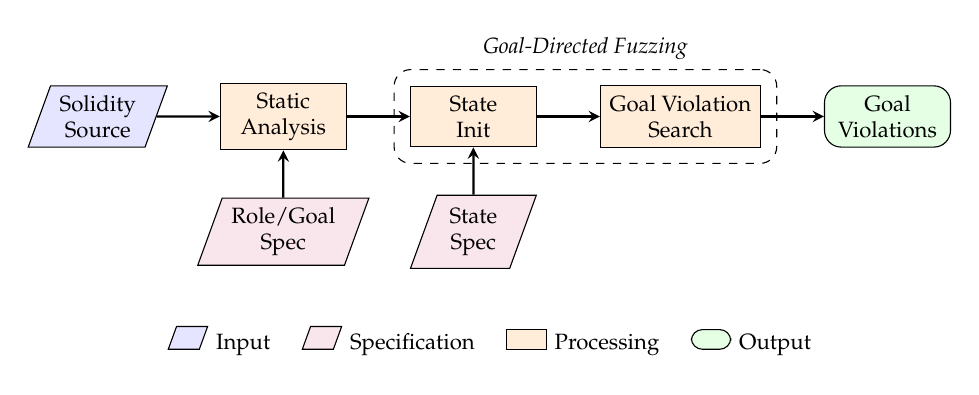
\begin{tikzpicture}[
    node distance=0.4cm and 0.8cm,
    % Base styles
    basebox/.style={minimum width=1.6cm, minimum height=0.6cm, align=center, font=\footnotesize},
    % Parallelogram for inputs/specs (slanted)
    inputbox/.style={basebox, draw, fill=blue!10,
        trapezium, trapezium left angle=70, trapezium right angle=110},
    specbox/.style={basebox, draw, fill=purple!10,
        trapezium, trapezium left angle=70, trapezium right angle=110},
    % Rectangle for processes
    processbox/.style={basebox, rectangle, draw, fill=orange!15},
    % Rounded rectangle for outputs
    outputbox/.style={basebox, rectangle, rounded corners=6pt, draw, fill=green!10},
    % Final output: double border
    finalbox/.style={basebox, rectangle, rounded corners=6pt, draw, fill=green!25, line width=1.5pt},
    % Arrow style
    arrow/.style={->, >=stealth, thick},
    % Legend styles
    legendpara/.style={draw, fill=#1, trapezium, trapezium left angle=70, trapezium right angle=110,
        minimum width=0.5cm, minimum height=0.25cm, inner sep=1pt},
    legendrect/.style={draw, fill=#1, rectangle, minimum width=0.5cm, minimum height=0.25cm},
    legendround/.style={draw, fill=#1, rectangle, rounded corners=4pt, minimum width=0.5cm, minimum height=0.25cm},
    legendfinal/.style={draw, fill=#1, rectangle, rounded corners=4pt, minimum width=0.5cm, minimum height=0.25cm, line width=1.2pt},
]

% Row 1: Input and Processing pipeline
\node[inputbox] (solidity) {Solidity\\Source};
\node[processbox, right=0.8cm of solidity] (static) {Static\\Analysis};
\node[processbox, right=of static] (stateinit) {State\\Init};
\node[processbox, right=of stateinit] (fuzzer) {Goal Violation\\Search};
\node[outputbox, right=of fuzzer] (violations) {Goal\\Violations};

% Specs below their corresponding processes
\node[specbox, below=0.6cm of static] (goalspec) {Role/Goal\\Spec};
\node[specbox, below=0.6cm of stateinit] (statespec) {State\\Spec};

% Arrows: inputs to static analysis
\draw[arrow] (solidity) -- (static);
\draw[arrow] (goalspec) -- (static);  % now vertical, spec below process

% Container: Goal-Directed Fuzzing (encapsulates State Init and Goal Violation Search)
\node[draw, dashed, rounded corners=6pt, inner sep=0.2cm, fit=(stateinit)(fuzzer),
      label={[font=\footnotesize\itshape, anchor=south]above:Goal-Directed Fuzzing}] (gdfcontainer) {};

% Arrow: state spec to state initialization
\draw[arrow] (statespec) -- (stateinit);

% Arrows: main pipeline flow
\draw[arrow] (static) -- (stateinit);
\draw[arrow] (stateinit) -- (fuzzer);
\draw[arrow] (fuzzer) -- (violations);

% Legend - below diagram, centered
\node[anchor=north, yshift=-0.6cm] at (current bounding box.south) {
    \footnotesize
    \begin{tabular}{@{}c@{\hspace{0.1cm}}l@{\hspace{0.4cm}}c@{\hspace{0.1cm}}l@{\hspace{0.4cm}}c@{\hspace{0.1cm}}l@{\hspace{0.4cm}}c@{\hspace{0.1cm}}l@{}}
        \tikz\node[legendpara=blue!10] {}; & Input &
        \tikz\node[legendpara=purple!10] {}; & Specification &
        \tikz\node[legendrect, fill=orange!15] {}; & Processing &
        \tikz\node[legendround, fill=green!10] {}; & Output
    \end{tabular}
};

\end{tikzpicture}
\caption{Architecture overview of \spoilsport.}
\label{fig:spoilsport-architecture}
\end{figure}


\subsection{Architecture Overview}
We present the overall workflow in \autoref{fig:spoilsport-architecture}.
\spoilsport takes the solidity source code of the target contract and the role/goal specification as input.
In addition, \spoilsport also takes the specification of state characteristics using role/goal semantics for its state initialization stage.

As final output, it delivers goal violating transaction sequences.

The pipeline consists of three processing stages:
\begin{enumerate}
    \item \textit{Static Analysis} extracts function-level summaries to guide the fuzzer.
    \item \textit{State Initialization} finds meaningful starting states using the user-provided state characteristics specification.
    \item \textit{Goal Violation Search} performs goal-directed fuzzing from the starting state to find violating transaction sequences.
\end{enumerate}

In the following, we discuss the key components of \spoilsport in detail. 

\subsection{Specification of Roles and Goals}
Rather than traditional bug or vulnerability test oracles which target bugs and vulnerabilities, we use role/goal semantics to specify user perspectives.
The reasons are two-fold. 
The first is that role/goal attribution localizes the violation to the user rather than a particular part of the program.
The second is that user desires are often naturally expressed as optimization problems or capabilities of calling particular functions, rather than binary properties.
Internally, \spoilsport does convert specified goals into properties which are checked for violation.

We allow for specifications of binary goals (\textit{does something happen?}), optimization goals (\textit{can I increase this value?}) and call capability goals (\textit{I want to be able to call this function}).


\smallskip
\noindent
\textbf{Roles and Goals for Goal Violation Search:}
We keep the roles and goals general enough to reasonably represent ERC-20 users without specifically accounting for heterogenous contract behavior.
This is to demonstrate that no special tailoring is required for this to find useful rug pull mechanics.

There are two roles involved in this analysis.
The first is a generic \holder role, which is defined as any user whose address is a key in the contract's \texttt{balances} variable.
This mapping variable is a frequently implemented pattern which associates user addresses to unsigned integers which track the amount of tokens they own.
However, such mappings default all keys to a value of $0$, making every user trivially a \holder.
The second is the \owner role, defined as the user who deploys the smart contract.
Internally, we develop a domain-specific language for \spoilsport and specify \holder as \texttt{balances[AddressUser] >= 0} and for the \owner as \texttt{AddressUser == AddressDeployer}.
The roles and goals are specified in 42 lines of Python code.

For the \textit{Token Holder} role, we specify the following goals:
\begin{enumerate}
    \item \textit{\rev{\maxowned}}: $\max$ \texttt{balances[AddressUser]}.
        This optimization goal captures the profit-maximizing goal of a user, which is to own as much value (measured in tokens) as possible.
    \item \textit{\rev{\minsupply}}: $\min$ \texttt{totalSupply}.
        Like the previous one, this optimization goal is  a profit-maximizing goal, capturing the intuition that a lower token supply increases the value of each individual token due to increased rarity.
    \item \textit{\liquidity}: $s \leadsto\texttt{AddressUser.transfer(balances[AddressUser])}$.
        This call capability goal captures the natural user expectation that they have full control over spending the tokens which they own.
        We define this as a user being able to transfer their full holdings to any other user, at any point from the start of analysis.
\end{enumerate}

Additionally, we exclude goal violations where a user reduces their own holdings (naively violating \maxowned{}), specified through the constraint \texttt{UserCaller != UserAddress}.
This is in keeping the principle behind \liquidity{}, which is that end-users should have control over their funds.
We also filter out \maxowned goal violations which use the \texttt{transferFrom()} function as their terminal function as these violations are generally trivial and consented to.
The \texttt{transferFrom()} function is typically used by a user who has been approved by the \holder to spend their funds.

We specify the following goal for the \textit{Contract Owner} role:
\begin{enumerate}
    \item \textit{\rev{\maxsupply}}: $\max$ \texttt{totalSupply}.
        Similar to \minsupply{}, this optimization goal is also a profit-maximizing goal but from the perspective of the entire project's value rather than a single user's holdings.
        This captures the intuition that creating more tokens will increase the market capitalization of the project (though this relationship is non-linear and subject to market dynamics).
\end{enumerate}



\textbf{State Characteristics for \textit{State Initialization}:}
We specify initial state characteristics which mimic real-world usage of rug pull contracts.
This is done in in 27 lines of Python code.
These capture the following scenario: tokens are disbursed among multiple users, and that at least one of those users is liquid.
As these are characteristics over groups of users, we extend the role/goal semantics by adding quantifiers over goals.
The characteristics are as follows:
\begin{enumerate}
    \item \textit{Disbursal:}
        $\forall u \in \text{\holder}$, \texttt{balances[u] >= 1000}.
        This ensures token disbursal of at least 1000 tokens to each user, creating multiple \holder{}.
    \item \textit{Any Liquidity:}  At least one \holder is liquid. Therefore, 
    $\exists u \in \text{\holder}$ where $s \leadsto\texttt{AddressUser.transfer(balances[u])}$.
       We note the deliberate choice to not make all users liquid, as many rug pull implementations are designed to disallow non-privileged users from transferring their funds.
\end{enumerate}

\subsection{Static Analysis}
We first generate function-level summaries which capture the following information:
\begin{enumerate}
    \item \textit{Write variables:} State variables which the function modifies.
    \item \textit{Control-flow variables:} State variables which are involved in conditionals and \texttt{require}/\texttt{assert} statements.
    \item \textit{Parameter types:} Type information for function parameters
\end{enumerate}

Additionally, on a contract-level, we save all hardcoded addresses present in the source code.
These are often used to encode privileged addresses such as admin wallets and fee recipients.
These addresses are used as concrete users during fuzzing.

\subsection{Goal-Directed Fuzzing}

\begin{algorithm}[!htb]
\caption{Fuzzing loop for \textit{Goal Violation Search}}
\label{ss:code:fuzz}
\KwIn{Static function summaries $\mathit{fn\_summaries}$, target goal $\mathit{goal}$, initialization sequence $\mathit{init\_seq}$}
\KwOut{Set of goal-violating transaction sequences}

$\mathit{testnet} \gets \textsc{InitTestnet}()$\;
$\mathit{queue} \gets$ new Queue()\;
$\mathit{candidates} \gets \textsc{GetFnsWritingToStateVars}(\mathit{fn\_summaries}, \mathit{goal.state\_vars})$\;

\ForEach{$\mathit{candidate} \in \mathit{candidates}$}{
    $\mathit{init\_seed} \gets$ Seed([$\mathit{candidate}$])\;
    $\mathit{queue}.\textsc{Add}(\mathit{init\_seed})$\;
}

$\mathit{solutions\_trie} \gets$ new SolutionTrie()\;

\While{$|\mathit{queue}| > 0$}{
    $\mathit{seed} \gets \mathit{queue}.\textsc{PopNextCandidate}()$\;
    \If{$\mathit{solutions\_trie}.\textsc{OverlapWith}(\mathit{seed})$}{
        \textbf{continue}\;
    }

    $\mathit{is\_success} \gets$ False\;
    $\mathit{solution} \gets$ None\;

    $\mathit{testnet}.\textsc{RunSequence}(\mathit{init\_seq})$\;
    $\mathit{baseline} \gets \textsc{CheckGoal}(\mathit{testnet}, \mathit{goal})$\;

    \ForEach{$\mathit{sequence} \in \textsc{Concretize}(\mathit{seed})$}{
        $\mathit{testnet}.\textsc{RunSequence}(\mathit{sequence})$\;
        $\mathit{is\_success} \gets \textsc{CheckGoalViolation}(\mathit{testnet}, \mathit{goal}, \mathit{baseline})$\;
        \If{$\mathit{is\_success}$}{
            $\mathit{solution} \gets \mathit{sequence}$\;
            \textbf{break}\;
        }
    }

    \eIf{$\mathit{is\_success}$}{
        $\mathit{solutions\_trie}.\textsc{Add}(\mathit{solution})$\;
    }{
        $\mathit{target\_fn} \gets \mathit{seed}.\textsc{GetFirstUnresolvedFn}()$\;
        $\mathit{prepend\_cands} \gets \textsc{GetFnsWritingToCfDeps}(\mathit{fn\_summaries}, \mathit{target\_fn})$\;
        \ForEach{$\mathit{prepend\_cand} \in \mathit{prepend\_cands}$}{
            $\mathit{new\_seed} \gets \mathit{seed}.\textsc{Copy}()$\;
            $\mathit{new\_seed}.\textsc{Prepend}(\mathit{prepend\_cand})$\;
            $\mathit{queue}.\textsc{Add}(\mathit{new\_seed})$\;
        }
    }
}

\Return $\mathit{solutions\_trie.solutions}$\;
\end{algorithm}

We now detail the fuzzing \revs{loops} which underlies \textit{State Initialization} and \textit{Goal Violation Search}.
These loops are heavily similar, with pseudocode of the \textit{Goal Violation Search} loop found in \autoref{ss:code:fuzz}.
Once state initialization transaction sequence is found, it is applied prior to our search for goal violations.

In \spoilsport, we treat seeds as a mix of transactions with concretized functions, and transactions with 
unconcretized functions which leave their arguments and caller unspecified.

We direct the fuzzer to satisfy the specified goals during \textit{State Initialization} as these are interpreted as desired state characteristics to search for.
Inversely, we direct the fuzzer to violate the specified goals during the \textit{Goal Violation Search}.
While we use the same seed generation and seed mutation phases across these stages, we use more complex seed scheduling for \textit{State Initialization} 
as it involves directing the fuzzer with multiple goals.

\smallskip
\noindent
\textbf{Seed generation:}
\revs{This is shown in lines 3-7 of \autoref{ss:code:fuzz}.}
We parse the goal specification to retrieve relevant state variables.
\revs{
    For instance, in searching for a \maxowned goal violation of \textit{MrMr} motivating example, we retrieve the \texttt{balanceOf} state variable.
}
We then populate our initial corpus with single unconcretized function calls of functions which modify these relevant state variables, based on our function summaries.
\revs{
    For \textit{MrMr}, these include \texttt{transfer()}, \texttt{transferFrom()} and \texttt{\_mints()}.
    As any goal violations necessarily have to modify relevant state variables, all possible goal violating seeds must terminate with a call to one of these functions.
}

\smallskip
\noindent
\textbf{Seed mutation:}
This is shown in lines 17-36 of \autoref{ss:code:fuzz}.
We attempt to execute a seed by sampling its unconcretized function parameters. 
\revs{
    If a seed fails to execute, we create a set of new seeds which prepend candidate functions that may make it succeed.
    These candidates are functions which are shown in the function summaries to write to control flow variables of the seed's failing function.
    For instance, if \texttt{transferFrom()} fails and depends on the \texttt{\_allowances}, the \texttt{increaseAllowance()} and \texttt{decreaseAllowance()} functions will be prepended as they write to \texttt{\_allowances}.
}
If a seed fails to execute, we extend it by prepending candidate enabling transactions.
These candidates are functions which modify the variables which the failing transaction's control-flow depends on.
This uses a similar insight to~\cite{ethploit}, constructing a transaction sequence from back to front.

\smallskip
\noindent
\textbf{Seed scheduling:}
This is implicit in line 10 of \autoref{ss:code:fuzz}.
We implement a round-robin approach to rotate between unconcretized function candidates.
In addition, during \textit{Goal Violation Search}, we employ a simple breadth-first search to prioritize shorter transaction sequences.
This is due to us \revs{fuzzing} for the violation of only a single goal at a time.
However, during \textit{State Initialization}, we augment this breadth-first search by prioritizing the seeds which have \revs{satisfied} the most goals.
For instance, a transaction sequence of length five which has \revs{satisfied} three goals would get precedence over a transaction sequence of length 4 which has \revs{satisfied} two goals.


\smallskip
\noindent
\textbf{Relation to Rug Pull Detectors:}
Our task of enriching a dataset of known rug pulls is complementary but distinct from the rug pull detection task of detectors such as Pied Piper~\cite{pied-piper} and TokenAuditor~\cite{tokenauditor_qrs22}.
Instead of identifying rug pulls, we are enriching understanding of already known rug pulls to surface transaction sequence examples of potential abuse and potentially detect unlabelled rug pull features.
Additionally, our approach is methodologically distinct in that we do not pre-specify patterns of rug pull behavior.
Given these task and methodological differences, comparison with existing rug pull detectors is difficult.


\section{Evaluation Setup}
\label{ss:sec:evaluation_setup}

\smallskip
\noindent
\textbf{Research Questions:} We answer the following research questions:

\smallskip
\textbf{RQ1 (State Initialization)}
How well does \spoilsport find meaningful starting states on rug pull smart contracts?

\smallskip
\textbf{RQ2 (Correlation with Known Rug Pull Types:)}
In searching for goal violations, does \spoilsport also uncover the root causes of rug pulls?

\smallskip
\textbf{RQ3 (New Information of Rug Pull Mechanisms:)}
Do the found goal violations effectively disclose new information about rug pull mechanisms in their contracts?

\smallskip
\textbf{RQ4 (Ablation of Control Flow Guidance)}
How much does the control flow guidance contribute to finding state initialization and goal violations?


\smallskip
\textbf{RQ1} investigates the efficacy of finding sequences of transactions to transform the smart contract states into ones which resemble characteristics of expected usage.
\textbf{RQ2} and \textbf{RQ3} inspect the relationship between found goal violations and trap doors in rug pulls.
Our evaluation does not aim to detect rug pulls in the wild, but rather enrich the ground truth of contracts which are %known to be 
malicious.
In \textbf{RQ2}, we present goal violation results and investigate whether these violations correspond to the dataset's labelled rug pull types.
In \textbf{RQ3}, we investigate the goal violations in more detail.
While our dataset gives us a high-level classification of the rug pull trap door, we wish to understand whether there is useful additional detail about rug pull mechanics which we may retrieve from goal violations.
In \textbf{RQ4}, we evaluate the efficacy of using the function-level control flow dependencies to guide seed mutation by removing this guidance.

\smallskip
\noindent 
\noindent \textbf{Heuristic-based detection of key variables:}
    We implement a heuristic-driven detection methodology for the key variables of the \texttt{balances} mapping variable (tracking user token holdings) and \texttt{totalSupply} variable (the sum of all issued tokens), which may take arbitrary names.
    This is loosely adapted from prior work~\cite{fairchecker}.
    We make use of functions mandated by the ERC-20 specification~\cite{ERC20TokenStandard}.
    For \texttt{balances}, we retrieve the type-matched variable which is read by \texttt{balanceOf()} and written by \texttt{transfer()}.
    If no candidate exists, we additionally check for a variable named \texttt{balanceOf} as that would result in an implicit \texttt{balanceOf} function.
    For \texttt{totalSupply}, we retrieve the type-matched variable which is read by \texttt{totalSupply()} and written by \texttt{transfer()}.
    If no candidate exists, we additionally check for a variable named \texttt{totalSupply} as that would result in an implicit \texttt{totalSupply} function.



\smallskip
\noindent
\textbf{Setup for evaluation:}
We use a dataset from prior work on rug pulls~\cite{SoKRugPull2025}, labelling 2,391 known rug pull contracts under their proposed root cause taxonomy.
\autoref{ss:fig:dataset-filtration} illustrates our process of filtering to the 1,376 (57.5\%) contracts used for our evaluation.
Of these, 2,279 have Solidity source code available from Etherscan~\cite{etherscan}.
As we only define roles and goals for ERC-20 smart contracts, we filter these to ERC-20 contracts only (2,002 contracts).
To generalize our specification of roles/goals across contracts, we use heuristic-based detection of required key variables, leaving us with 1,680 contracts.
Additionally, our fuzzer does not currently support contracts which perform function calls to external dependencies.
This leaves us with a final 1,376 contracts for our evaluation.
We allocate a time budget of 30 seconds per contract.

\begin{figure}[h]
\centering
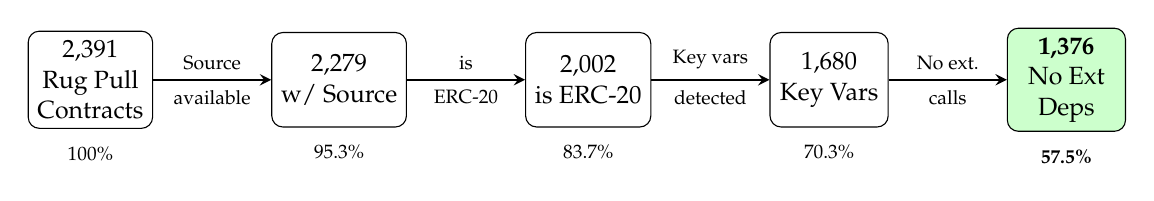
\begin{tikzpicture}[
    node distance=1.5cm,
    box/.style={rectangle, draw, rounded corners, minimum height=1.2cm, minimum width=1.5cm, align=center, font=\small},
    arrow/.style={->, thick, >=stealth},
    lbl/.style={font=\scriptsize}
]
% Boxes
\node[box] (start) {2,391\\Rug Pull\\Contracts};
\node[box, right=of start] (source) {2,279\\w/ Source};
\node[box, right=of source] (erc20) {2,002\\is ERC-20};
\node[box, right=of erc20] (keys) {1,680\\Key Vars};
\node[box, right=of keys, fill=green!20] (final) {\textbf{1,376}\\No Ext\\Deps};

% Arrows with split labels (above and below)
\draw[arrow] (start) -- (source) node[midway, above, lbl] {Source} node[midway, below, lbl] {available};
\draw[arrow] (source) -- (erc20) node[midway, above, lbl] {is} node[midway, below, lbl] {ERC-20};
\draw[arrow] (erc20) -- (keys) node[midway, above, lbl] {Key vars} node[midway, below, lbl] {detected};
\draw[arrow] (keys) -- (final) node[midway, above, lbl] {No ext.} node[midway, below, lbl] {calls};

% Percentage labels below boxes
\node[below=0.1cm of start, font=\scriptsize] {100\%};
\node[below=0.1cm of source, font=\scriptsize] {95.3\%};
\node[below=0.1cm of erc20, font=\scriptsize] {83.7\%};
\node[below=0.1cm of keys, font=\scriptsize] {70.3\%};
\node[below=0.1cm of final, font=\scriptsize] {\textbf{57.5\%}};
\end{tikzpicture}
\caption{Dataset filtration pipeline for rug pull evaluation.}
\label{ss:fig:dataset-filtration}
\end{figure}


The dataset labels are high-level, specifying the kind of root cause of the rug pull as well classifying its type.
This does not allow for reproduction of the exact mechanism of the rug pull (i.e., it does not identify which functions or transactions were used to actuate the fraud).
As in the full dataset, the trap door labels in this sample are heavily skewed towards \textit{Transaction Limitation} violations (97.7\% of all entries).
Of these, 95.3\% are due to \textit{Sale-Restrict} which only allows privileged users to transfer their tokens, 3.1\% are due to \textit{Freeze Account} which prevent victim wallet addresses from performing transactions and
1.4\% are due to \textit{Transfer Block} which globally disables transfers.

\smallskip
\noindent 
\textbf{Optimizations:} To speed up the construction of transaction sequences, we implement the following optimizations:
\begin{enumerate}
    \item \textit{Initial corpuses optimizations:}
        To prioritize values at sign boundaries, we used initial corpuses of $\{-1, 0, 1\}$ for unsigned integer parameters and $\{0, 1\}$ for signed integer parameters.
        Once exhausted, random values based on bitwidth are generated.
        This is to prevent overshooting when conditionals bound input values.
        We also constrained address parameters to select from the available bounded address space only.
        Additionally, we retrieve any constant values from goal specification and inject those into the initial corpus.
    \item \textit{Bounded address space:}
        While addresses are normally 160-bit values, we constrain them to a small set with an adjustable parameter.
        During our static analysis stage, we retrieve hardcoded addresses from the Solidity source code as these are common in rug-pull contracts (e.g., used to encode privileged addresses).
    \item \textit{Revm testnet backend:} 
        We integrated the following EVM implementations as testnet backends for \spoilsport: Ethereum Tester~\cite{ethereum_tester}, Anvil~\cite{anvil} with JSON RPC and Revm~\cite{revm} with rust bindings to python.
        Of the three, the Revm integration was fastest at 6,962 transactions per second (TPS).
        Anvil and Ethereum Tester were significantly slower, with 91TPS and 44TPS respectively.
        We use the Revm integration for experiments as it is two orders of magnitude faster.
\end{enumerate}

\smallskip
\noindent
\textbf{\spoilsport configuration:}
We dynamically configure the number of users in our bounded address space to $\max{(hardcoded_{addresses} + 2, 3)}$.
This ensures that all hardcoded addresses are available as users while also including non-hardcoded users to represent typical end-users.
\todo{Did we talk about a solver? I think readers will be confused where the solver is playing a role for fuzzing.} For every function evaluated, 
we configure the solver to generate test input corresponding to the cartesian product of five values per parameter across all potential users as transactors.

During the \textit{State Initialization} step, we limit the maximum transaction sequence size to 20.
Additionally, we bias the initial contract deployer user to be a non-hardcoded address to increase realism.
During the \textit{Goal Violation Search} step, we limit the maximum transaction sequence size to two.
This is due to the majority of rug pull features identified in literature~\cite{trapdoor,SoKRugPull2025,pied-piper} requiring at most two transactions.


\smallskip
\noindent
\textbf{Frameworks and Platforms:}
We retrieve smart contract source code from Etherscan~\cite{EthMarketCap}.
During our \textit{Static Analysis} stage, we use Slither~\cite{Slither} to construct function summaries which contain data and control flow dependencies.
We use the Revm \cite{revm} Ethereum Virtual Machine (EVM) implementation as our execution backend.
The majority of the code is written in Python, with custom Rust bindings for Revm written in PyO3.
All evaluations were conducted on a 16-inch Macbook Pro (2021 model, M1 Max CPU).

\section{Results}
\label{ss:sec:results}

\smallskip
\noindent
\textbf{RQ1 (State Initialization):}



\begin{table}[h]
\centering
\caption{State initialization timing statistics (in seconds).}
\label{tab:rq1-timing}
\begin{tabular}{@{}lrrrrr@{}}
\toprule
& Mean & Median & Min & Max & Std \\
\midrule
Time (s) & 1.54 & 0.52 & 0.03 & 29.73 & 3.83 \\
\bottomrule
\end{tabular}
\end{table}

\spoilsport successfully initialized 1,324 of 1,376 (96.3\%) ERC-20 contracts with a timeout of 30 seconds.
\autoref{tab:rq1-timing} summarizes the timing statistics, showing a quick mean time (1.54s).

Of the 51 failures (3.7\%), 38 contracts (74.5\% of failures) were due to the solver timing out.
An further 13 contracts (25.5\% of failures) failed due to issues accessing or identifying the \texttt{balances} variable.

As shown in \autoref{ss:fig:rq1-init-length-distro} lengths ranged from two to twelve transactions, with the most frequent being lengths of three (940 contracts, 71.1\%), five (164 contracts, 11.9\%) and four (98 contracts, 7.1\%).
The vast majority (1,316, 98.9\%) of these sequences consisted solely of \texttt{transfer} calls.
This is consistent with the general pattern of all token being minted to a single address upon deployment, and that address then disbursing the funds.

\begin{figure*}[h]
	\centering
	\includegraphics[width=0.9\linewidth]{img/rp_state_init_sequence_length_distribution.png}
	\caption{Distribution of transaction sequence lengths for found state initialization sequences.}
	\label{ss:fig:rq1-init-length-distro}
\end{figure*}



\begin{figure}[h]
\centering
\resizebox{\linewidth}{!}{%
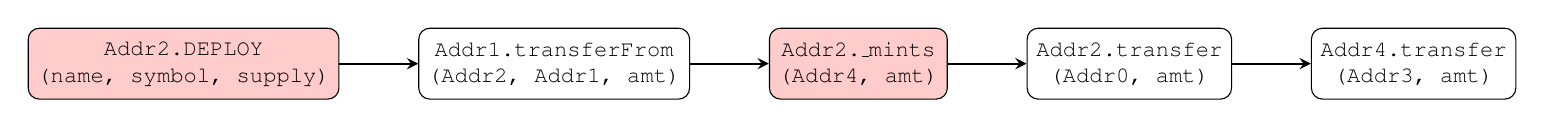
\begin{tikzpicture}[
    node distance=1cm,
    txstep/.style={rectangle, draw, rounded corners, align=center, font=\footnotesize, minimum width=1.6cm, minimum height=0.9cm},
    call/.style={->, >=stealth, thick}
]
    % Each node shows Caller.function\n(args)
    \node[txstep, fill=red!20] (s1) {\texttt{Addr2.DEPLOY}\\\texttt{(name, symbol, supply)}};
    \node[txstep, right=of s1] (s2) {\texttt{Addr1.transferFrom}\\\texttt{(Addr2, Addr1, amt)}};
    \node[txstep, right=of s2, fill=red!20] (s3) {\texttt{Addr2.\_mints}\\\texttt{(Addr4, amt)}};
    \node[txstep, right=of s3] (s4) {\texttt{Addr2.transfer}\\\texttt{(Addr0, amt)}};
    \node[txstep, right=of s4] (s5) {\texttt{Addr4.transfer}\\\texttt{(Addr3, amt)}};

    % Arrows
    \draw[call] (s1) -- (s2);
    \draw[call] (s2) -- (s3);
    \draw[call] (s3) -- (s4);
    \draw[call] (s4) -- (s5);
\end{tikzpicture}%
}
\caption{Example non-standard state initialization transaction sequence for the \textit{MrMr} token, with each node corresponding to a transaction.
The red nodes make use of rug pull mechanics.}
\label{ss:fig:rq1-mrmr-flow}
\end{figure}

In \autoref{ss:fig:rq1-mrmr-flow}, we highlight an example of a non-standard state initialization sequence found in the \textit{MrMr} contract (\texttt{0x01{\allowbreak}bcc8{\allowbreak}8d1b{\allowbreak}62e9{\allowbreak}7f9b{\allowbreak}d6a0{\allowbreak}58d1{\allowbreak}f442{\allowbreak}226a{\allowbreak}234ea3}) to show the generality of the state initialization search.
Here, the \owner{}'s (\textit{Address2}) deployment implicitly blocks all transfers that are not by themselves or a particular hardcoded address (\textit{Address1}) and mints themselves the initial token supply.
\textit{Address1} then calls a misleading \texttt{transferFrom} function, which succeededs because it passes the two checks of being whitelisted and transferring to the \owner.
The \owner then uses the misleadingly-named \texttt{\_mints()} function to whitelist \textit{Address4}, allowing it to transfer tokens, and overwrites its balances with a large amount rather than minting tokens.
This balance overwriting is covert and does not modify \texttt{totalSupply}.
\texttt{Address2} and \texttt{Address4} then transfer tokens to the remaining two users.
Our solver has now found a novel path which exploits rug pull mechanics to meet the target characteristics of token disbursal with at least one liquidity user.

This demonstrates that the declarative state specification using role/goal semantics is effective (96.3\% success) and efficient (median 0.52 seconds) for large-scale analysis, even in the adversarial setting of compromised ERC-20 contracts found in the wild.

\begin{result}
    \spoilsport successfully initialized 96.3\% (1,324) ERC-20 contracts quickly (mean 1.54s).
\end{result}
\smallskip
\noindent
\textbf{RQ2 (Correlation with Known Rug Pull Types):}

% \begin{figure*}[h]
% 	\centering
% 	\includegraphics[width=\linewidth]{img/rp_violations_by_goal_no_mot.png}
% 	\caption{Counts of goal violations found by \spoilsport{} in the rug pull dataset, broken down by goal.}
% 	\label{ss:fig:rq2-violations-by-motivation}
% \end{figure*}

\begin{table}[h]
\centering
\caption{Goal violations found by \spoilsport{} on rug-pull contracts (n=1,324).}
\label{ss:table:rq2}
\begin{tabular}{|c|c|c|c|c|c|}
\hline
\textbf{Role} & \textbf{Goal} & \textbf{\# Viol.} & \textbf{\# Viol.} & \textbf{Time} & \textbf{Avg Time} \\
              &               & \textbf{Contracts} & & & \textbf{/ Viol.} \\
\hline
\multirow{3}{*}{\holder}
    & \maxowned  & 81 (6\%) & 402   & 3h 4m & 27.4s \\
\cline{2-6}
    & \minsupply & 978 (71\%) & 982   & 39.8s & <0.1s \\
\cline{2-6}
    & \liquidity & 1,155 (84\%) & 1,283 & 4h 19m & 12.1s \\
\hline
\owner & \maxsupply & 40 (3\%) & 64 & 44m & 40.8s \\
\hline
\multicolumn{2}{|l|}{\textbf{TOTAL}} & \textbf{1,257 (91\%)} & \textbf{2,731} & \textbf{8h 7m} & \textbf{10.7s} \\
\hline
\end{tabular}
\end{table}

In \autoref{ss:table:rq2}, we present goal violations detected from the 1,324 rug pull contracts that were successfully initialized in \textbf{RQ1}.
Overall, \spoilsport{} took a mean of 10.7s to find each of the 2,731 goal violations.
Across the labelled rug pull types, we find at least one goal violation in the corresponding goal for 83.6\% of contracts.
The largest number of violations found (1,155) was in \liquidity{}.
This reflects the dataset's original distribution, which is strongly dominated by \textit{Transaction Limitation}-based rug pulls.
This type works by limiting end-user transactions, generally to stop them from selling their tokens.

We found \liquidity violations in 1,143/1,303 (87.7\%) of the \textit{Transaction Limitation} rug pulls.
156 (12.0\%) of these contracts timed out before completing the goal violation search.
The majority of the violations i.e., %were attributed to the \owner calling \texttt{decreaseAllowance()}.
735 (73.6\%) %of these 
are caused by the \owner calling the \texttt{decreaseAllowance()} function.
This function name misleadingly implies that it implements the standard \textit{allowance} feature in 
ERC-20 specification~\cite{ERC20TokenStandard}. This should allow users to control who they permit 
to spend their funds. %Upon manual analysis, we 
Our analysis finds that it instead restricts all token transfers not made 
by a privileged address, appropriately setting up the \textit{Sale-restrict} scenario.

Though a small minority, we importantly fail to detect the labelled root causes of 6/9 (66.7\%) of the next 
most prominent rug pull type. This is \textit{Token Generation}, in which additional tokens are covertly generated.
This failure is largely attributed to how we specify the \minsupply goal \revs{(\textit{see} \autoref{ss:sec:overall_workflow})}, which hides 
the assumption that \texttt{totalSupply} variable accurately tracks the total token supply. Deceptively, the missed contracts 
tend to increase an attacker's owned tokens without correspondingly updating the \texttt{totalSupply} variable.
This highlights a flaw in our initial specification, which may in future be improved on to track the sum of all 
users' token holdings rather than the \texttt{totalSupply} variable.


\begin{results}
    83.6\% of the rug pull types had corresponding violated goals among the 2,731 general ERC-20 violations, validating that these goal violations are consistent with the original dataset's coarse classification.
\end{results}
\smallskip
\noindent
\textbf{RQ3 (New Information on Rug Pull Mechanisms):}
We note that it is difficult to classify some features cleanly as rug pull mechanisms.
For instance, the \texttt{decreaseAllowance()} function may be cleanly classified as a rug pull mechanic as its deceptive naming and implementation imply that it will be used fraudulently.
However, there are 12 contracts with transparently-named and correctly-implemented \texttt{pause()} functions which globally halt all token transfers, including those by the attacker.
This could be used to halt token transfers while the attacker drains the accumulated paired tokens from a decentralized exchange.
However, this is also a feature that is commonly found in ERC-20 contracts~\cite{chi-end-user} in general.
While nearly all found goal violations may be used to further rug pulls, we do not provide a clean classification for this reason.

\revs{
    Our manual analysis of the automatically discovered goal violating transaction sequences is aimed at identifying examples and details of how these rug pulls may be actuated.
    This enriches the initial dataset, which provides only high level classifications of rug pulls.
    To this end, these goal violations add
}
three interesting sources of information during analysis.

The first is whether the goal is already violated upon state initialization.
1,253 \textit{sale-restrict} contracts are labelled under the \textit{sale-restrict} root cause, which is effected by disallowing all non-privileged users from selling their tokens.
However, 90.4\% of these contracts were not immediately violated upon state initialization.
This informs us that such contracts are capable of allowing users to trade tokens normally prior to the attacker restricting sales.


\revs{
    The second is the functions used in goal violations, which provide information about rug pull patterns across contracts as well as localize suspicious behavior to particular functions within single contracts.
    Disregarding the particular arguments and callers, we note that the 1,104 \textit{sale-restrict} \liquidity violations come from only 16 different sequences of function calls.
    This immediately suggests high code-reuse or common rug pull patterns.
    Additionally, analyzing multiple goal violations within the same smart contract can reveal further detail.
}
For these \textit{sale-restrict} contracts, 105 of them each have two \liquidity violations of the \owner calling the non-standard function \texttt{transfernewun()} and any user role calling the seemingly-innocuous function \texttt{transferFrom()}.
Upon manual analysis, we note that the first call to \texttt{transferFrom()} restricts (blacklists) that first recipient from further reception through the \texttt{transfer} function, \revs{and that \texttt{transfernewun()} allows the \owner to change which address is blacklisted.}
The \texttt{transferFrom()} \revs{\texttt{blacklist}} implementation is particularly elegant because it keeps the on-chain data looking clean as calls to functions named \texttt{transferFrom} are not suspicious, and because it operates as an ordinary \texttt{transferFrom()} function after the first call.
This is misclassified under the dataset's taxonomy \revs{as a \textit{sale-restrict} root cause rather than a \textit{whitelist/blacklist} root cause}.


\revs{
    The third is the roles involved in the goal violations, which may help understand how rug pulls hide suspicious features.
}
\revs{
    For instance, the caller of the prior \texttt{transferFrom()} function could in theory be any user, requiring only the \holder role.
    The lack of explicit access control helps to hide its \texttt{blacklist} behavior.
}
In practice, the first \texttt{transferFrom()} call is generally to a liquidity pair on a decentralized exchange (DEX).
This thus allows the owner to add liquidity and then prevent subsequent selling of tokens by preventing victim \holder{}s from selling their tokens to that DEX without restricting them from purchasing.
This then allows the owner to withdraw the accumulated purchase liquidity.
\revs{
    However, this introduces the concern that some unintended user will first \texttt{transferFrom()}.
    By noting that only \owner{} can call \texttt{transfernewun()}, we may understand that \texttt{transfernewun()} serves as an access-controlled contingency for the \owner to change the blacklisted address to the DEX in this case.
}

% The fourth is the motivation analysis.
% The \textit{Motivated} sequences signal that the underlying transactors' goals are aligned with the goal violations, making them particularly important to inspect.
% 964/989 of the \textit{Motivated} transaction sequences are \minsupply violations which allow the \owner to arbitrarily generate tokens.
% While these should be \textit{Token Generation} features, they are not labelled as such in the dataset.
% These use various levels of obfuscation to mislead end-users.
% Two of these are transparently named \texttt{mint()}, signalling token generation capability.
% 954 use the name of an internal, not publicly-accessible function (\texttt{\_mint()} in the frequently-used OpenZeppelin~\cite{OpenZeppelinContracts} ERC-20 implementation, but make it accessible.
% This makes the \texttt{\_mint()} functions seem innocuously inaccessible at first glance.
% Most misleadingly, six of these use function names which signal different behavior, such as \texttt{\_BURN()}, \texttt{blacklist()} and \texttt{work()}.


\begin{results}
    Goal violations enrich the dataset by revealing 105 misclassifications, reveal 964 unlabelled \textit{Token Generation}-type rug pull mechanics, and provide examples of rug mechanics being used.
\end{results}
\section{Discussion}
\label{ss:sec:discussion}


\smallskip
\noindent
\textbf{Avoiding dependence on particular features:}
By sticking purely to generic user roles and goals, we were able to avoid particularities of features during our rug pull analysis.
This is a fundamentally different approach to existing detectors, which index on known features~\cite{pied-piper,do-not-rug_math22}.
By avoiding fitting to these features, our approach may be robust to novel rug pull patterns which existing detectors may miss.
This is supported by our ability to detect rug pull concerns which were beyond the original dataset's labels, as shown in \textbf{RQ3}.
However, a trade off is that our found goal violations require manual inspection in order to understand.

% \todo
% \smallskip
% \noindent
% \textbf{Comorbidity of risky features:}
% \todo
% We note that many rug pull contracts have multiple features which would both violate user expectations as well as facilitate rug pulls.


\smallskip
\noindent
\textbf{Unclear classification of rug pulls based solely on features:}
While we examine many clearly hidden features that imply malice, we note that other more cleanly implemented features can only be classified as malicious or benign based on usage.
For instance, the USD Tether~\cite{TetherWhitepaper} contract, which houses the most popular ERC-20 smart contract, is centrally controlled by a single wallet with a \feature{mint} feature that allows it to generate an arbitrary amount of tokens.
This could be used to turn a rug pull-style quick profit by generating and then selling tokens, but this is unlikely due to other incentives and no abuse has ever been recorded.
Thus on an implementation-level, USD Tether has the necessary features to actuate a rug pull, yet by usage it is clearly not a rug pull.
This highlights the importance of surfacing risky features rather than cleanly classifying a smart contract as a rug pull or not after-the-fact.

\section{Related Work}
\label{ss:sec:related_work}

\subsection{Trap Door Rug Pulls}
A recent systemization of knowledge~\cite{SoKRugPull2025} develops an overarching rug pull taxonomy and compiles the dataset we use in this work.
Various works focus on detection of these rug pulls.
Similar to us, TokenAuditor~\cite{tokenauditor_qrs22} uses a fuzzing-based approach.
Pied Piper~\cite{pied-piper} first performs static analysis with datalog to detect trap door candidates and then validates them through directed fuzzing.
Several works~\cite{do-not-rug_math22,trade-or-trick_acs22,trapdoor} find rug pulls through heuristics and machine learning techniques.
Two of these works~\cite{do-not-rug_math22,trapdoor} center on tokens which were listed on Uniswap~\cite{uniswap_protocol}.
These works focus on particular features of rug pulls in order to unearth them.
However, our approach and tool look for general goal violations within ERC-20 contracts.
With the exception of the state initialization procedure, we do not tailor our search to rug pulls in particular.
This frees us from dependence on particular characteristics of rug pull smart contracts.

\subsection{Smart Contract Fuzzers and State Initialization}
Wu et al present a recent survey on smart contract fuzzers~\cite{fuzzer_survey_2024}.
Similar to us, several works use static and dynamic dataflow-based guidance~\cite{smartian_ase21,ethploit,ir-fuzz_ifs23} to construct targeted transaction sequences.
Additionally, many fuzzers use code coverage~\cite{sfuzz_icse20,ityfuzz_issta23,reguard} and branch distance~\cite{sfuzz_icse20,ir-fuzz_ifs23,ityfuzz_issta23} in order to prioritize interesting seeds. 
Combining fuzzing and symbolic execution, some works leverage symbolic analysis in order to solve difficult-to-reach constraints~\cite{ConFuzzius_eurosp21,ilf_ccs19}.
Other works employ machine learning techniques to guide transaction sequence generation~\cite{rlf_ase22,ilf_ccs19}.
In general, these fuzzers are oriented at discovering bugs and vulnerabilities, which is a distinct task from finding goal violations.
While these techniques are useful to improve our tool, our task required a custom fuzzer to tightly integrate the role/goal specification format, including optimization and call capabilitiy goals.
IR-Fuzz~\cite{ir-fuzz_ifs23} highlights that many fuzzers expend excessive energy around state initialization.
Similarly, our state initialization methodology is oriented at finding goal violations more efficiently.
However, our aim is to find usage-realistic initial states that are conducive to goal analysis, rather than conducive to finding bugs and vulnerabilities.

\subsection{Testing Beyond Traditional Bugs and Vulnerabilities in Smart Contracts}
There are two research directions which move beyond traditional bugs and vulnerabilities.
The first targets economic security, searching for profit-generating exploits~\cite{DeFiSoK2023,ClockworkFinance} rather than incorrect implementations.
The Clockwork Finance Framework~\cite{ClockworkFinance} employs formal techniques to compose user-defined models of the underlying mechanisms implemented through smart contracts in order to reason about their economic security properties.
Lanturn~\cite{Lanturn} uses adaptive learning directly on EVM bytecode to generate profitable transaction sequences.
The second research direction is in fairness verification.
Zeus~\cite{zeus_ndss18} searches for violations of specified business logic within implementations of smart contracts.
FairCon~\cite{fse20-fairness} uses properties from mechanism design literature to evaluate the fairness of auctions in DeFi.
FairChecker~\cite{fairchecker} proposes two general properties which detect if attackers may gain profit without cost.
Both directions have overlap with our task of finding end-user goal violations as what makes economic attacks and fairness violations concerning is that they violate end-user goals.
Our task differs from economic security as it is additionally concerned with non-economic goals, such as voting outcomes in DeFi governance.
It differs from fairness verification in that we are interested in identifying goal violations even if the underlying protocol is fair as end-users may not have accurate understandings of these protocols.
This is motivated by prior work~\cite{mentalmodel-soups,chi-end-user} which shows that end-users often misunderstand important mechanics of the blockchain and smart contracts.
\section{Threats to Validity}
\label{ss:sec:threats_to_validity}

\smallskip
\noindent \textbf{Limitations of the dataset:}
The original dataset is heavily skewed towards \textit{Transaction Limitation} (87\% of rug pulls)~\cite{SoKRugPull2025}.
After our filtering pipeline detailed in \autoref{ss:sec:evaluation_setup} and after excluding the 52 contracts which we failed to find initial state for, this skew increases to 98.3\%.
This limits the generalizability of our results to other rug pull types.
However, this is partially mitigated by our analysis in \textbf{RQ4}, which finds 964 non-\textit{Transaction Limitation} rug pull mechanics.
Additionally, this dataset was created from three composite datasets of other works~\cite{pied-piper,honeypot_usenix19,trapdoor}, implying that this may be representative of rug pull contracts.

\smallskip
\noindent
\textbf{Limitations of the goal violation discovery task:} 
    While this work demonstrates overlap, goal violations and rug pull mechanisms are not equivalent.
    As addressed in \autoref{ch:goalseeker}, there are legitimate purposes for goal violations which are not fraudulent.
    Further, end-users have subjective goals.
    While the specification is meant to be a reasonable stand in for this subjectivity, real-world end-user goals may differ from the specification.
    Additionally, ERC-20 contracts may have a wider diversity of roles.
    For instance, rug pull contracts often have rely on a router smart contract for integration with decentralized exchanges, which motivates a router role.
    Therefore the specification may be incomplete with respect to particular contracts.

\smallskip
\noindent
\textbf{Limitations of the \spoilsport solver:} 
We are primarily limited by our time budget and configuration of five candidates for each function parameter.
Additionally, we inherit the limitations of fuzzers in general, such as difficulty in finding test inputs which meet tightly-bounded conditions.
Specific to Ethereum, our fuzzer does not currently attempt different block timestamps for transactions.
This renders it difficult to find violations which are dependent on block timestamps.
Additionally, our solver does not support multi-contract analysis.
We therefore had to exclude 304 (12.7\% of) contracts which called external dependencies, introducing selection bias into our analysis.
\section{Conclusion}
\label{ss:sec:conclusion}
We demonstrate that an analysis of general ERC-20 user roles and goals in 1,376 known rug pull contracts automatically recovers and enriches many rug pull mechanics.
These perspectives are implemented in the role/goal semantics, without tailoring to particular rug pull patterns.
Overall, we found 2,731 goal violations with our custom \spoilsport goal-directed fuzzer, unveiling unlabelled and mislabelled mechanics which may be used to rug pull end-users.
Additionally, we develop a declarative methodology to find usage-realistic starting states from which to search for goal violations and define realistic state characteristics of ERC-20 rug pulls.
Using a dataset of known rug-pull contracts~\cite{SoKRugPull2025}, our evaluation shows that \spoilsport{} successfully initializes 1,324/1,376 (96.3\%) of our target contracts to these starting states.
Future work includes extending the \spoilsport fuzzer to handle multi-contract systems in order to better investigate financial fraud in more complex DeFi applications.
\section{Data Availability}
All source code and results are available at \url{https://anonymous.4open.science/r/spoilsport-fuzzer-0910}.
\section{Acknowldgements}
We disclose that Claude Code was used to aid in the development of some of the code underlying \spoilsport.
The authors take full responsibility for the generated code, having reviewed and tested it.

\balance
\bibliographystyle{ACM-Reference-Format}
\bibliography{main}


\end{document}